\chapter{Implementation}

\section{Camera module}

\modc{\subsection{Hardware connection}}

The Raspberry Pi camera module was connected to the Jetson TK1 board as shown \mdc{in} \fref{imp:schematic}\modc{ and \fref{imp:connection}}. A 74HCT245 bus transceiver chip was used as a buffer for voltage level conversion, since GPIOs on the Jetson board are using $1.8V$ voltage level while the Raspberry Pi module is working at $3.3V$ voltage level. \modc{The camera needs 2 discrete interfaces for control and \mdd{communication}, I2C and MIPI-CSI. I2C\mdd{, which is} a relatively low speed interface with multi master and multi slave addressing support, is used to control and configure the camera. MIPI-CSI is a high speed data transmission interface designed for high resolution cameras, by having multiple differential data lanes to multiple maximum transmission speed. The camera uses 2 data lanes to transmit frame data and synchronise.}

\begin{figure}[htb]
  \centering
  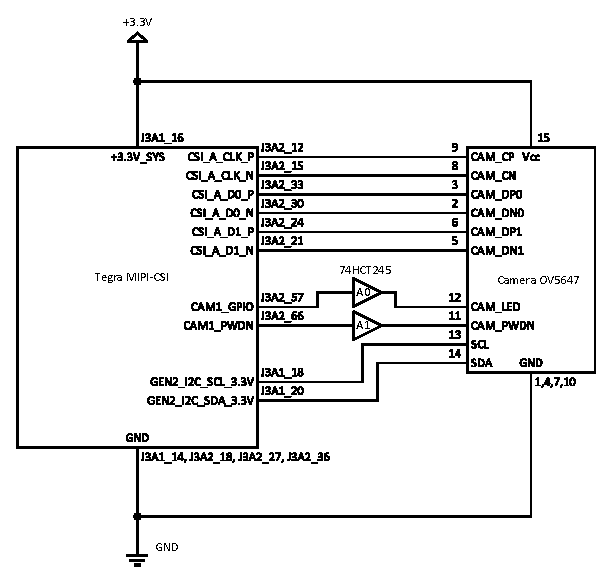
\includegraphics[width=0.7\columnwidth]{schematic}
  \caption{Schematic of Jetson board connect to a Raspberry Pi camera module.}
  \label{imp:schematic}
\end{figure}

\modc{\begin{figure}[htb]
  \centering
  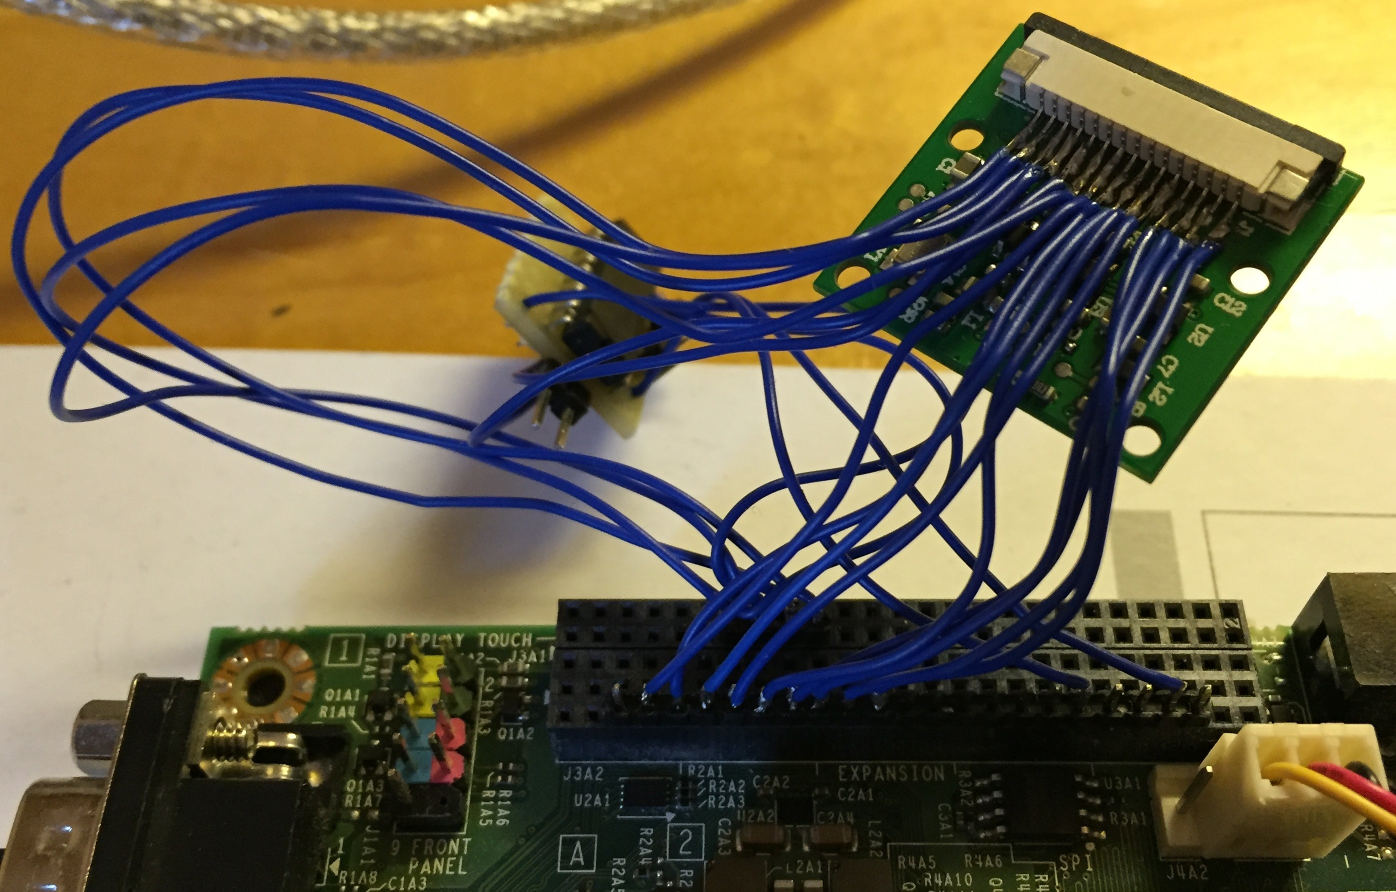
\includegraphics[width=0.7\columnwidth]{connection}
  \caption{Photo of the connection between the camera model and the Jetson board.}
  \label{imp:connection}
\end{figure}

The camera module is using an on-board $25$ MHz oscillator, multiplied to $48$ MHz pixel clock by Phase Locked Loop (PLL) inside the camera sensor. Alteration of frame interval was done by adding dummy blank lines after actual frame data.

The GPIO on the camera module is controlling \mdc{an} LED mounted on the module, and it is controllable through the camera driver. Therefore by controlling the GPIO, it not only \mdc{can give} indications about camera activity, but also is very useful for debugging and triggering external power analyser.

%{\color{red}Camera waveform.}

\fref{imp:cam:osc} shows a detailed waveform captured using an oscilloscope during camera frame rate configuration. The camera was configured to a higher resolution mode for 2 frames, then changed back. Frame data, line data, synchronisation packet and I2C transmissions are clearly marked on the waveform.

\begin{figure}[htb]
  \centering
  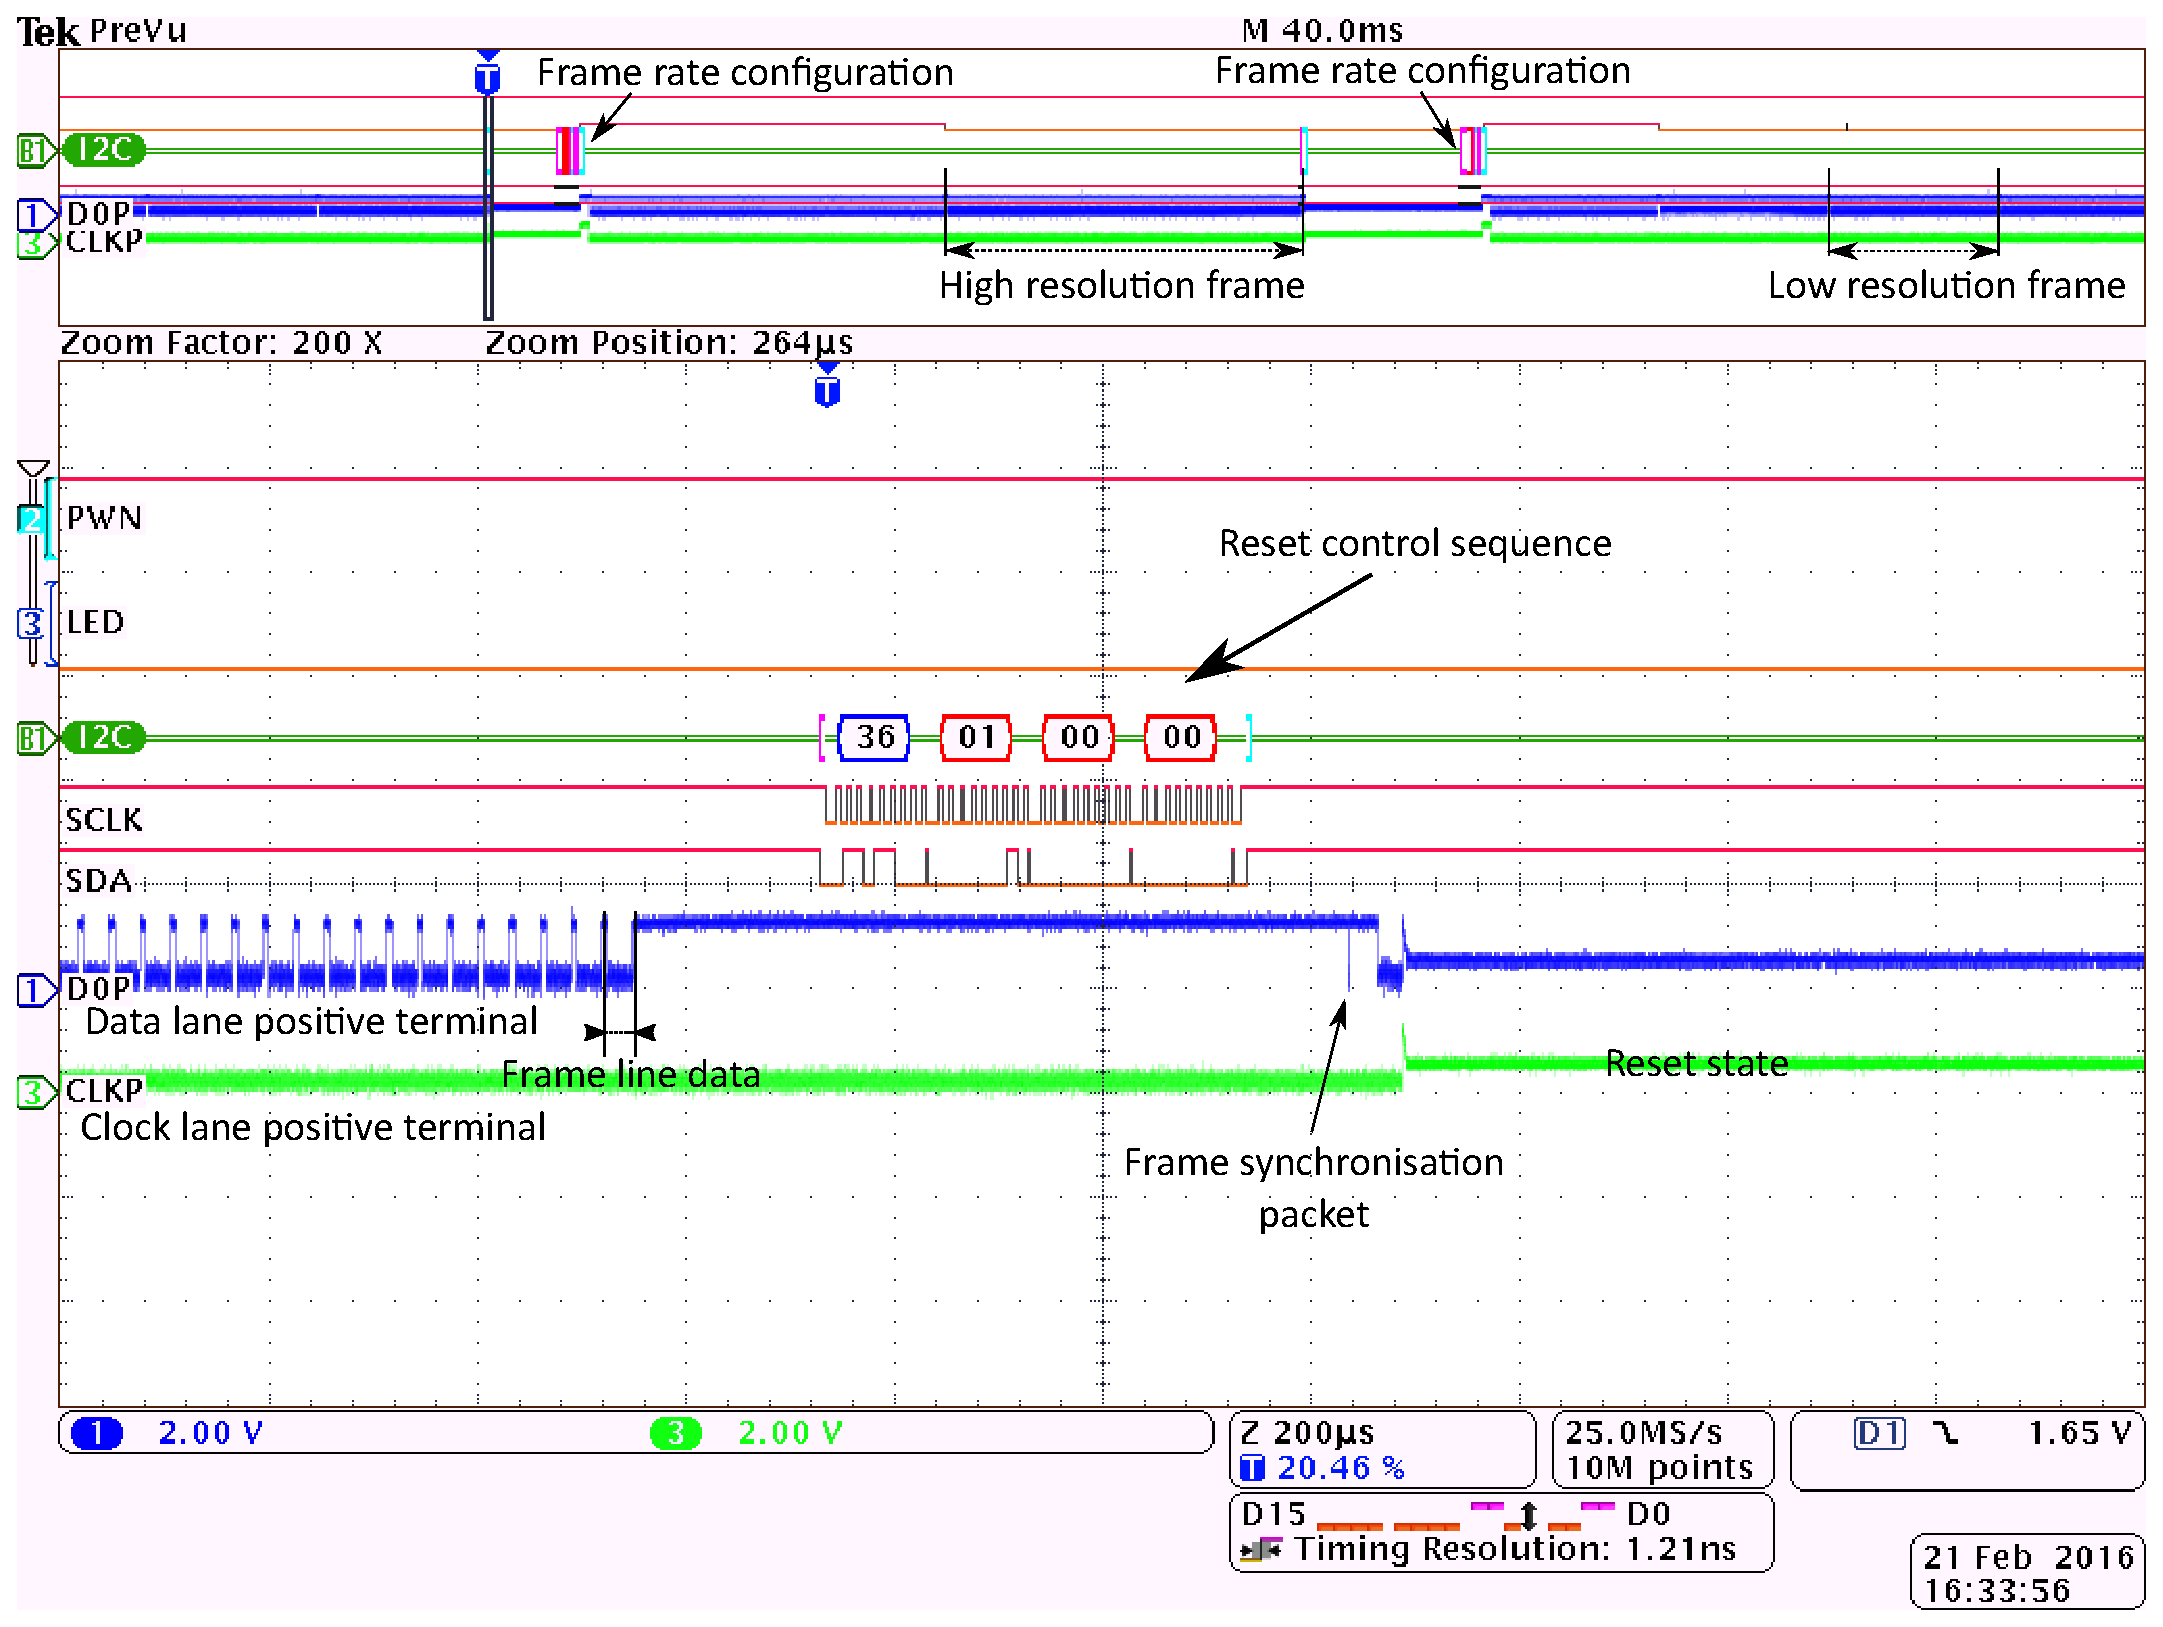
\includegraphics[width=\columnwidth]{cam_osc}
  \caption{Waveform capture of configuring camera module.}
  \label{imp:cam:osc}
\end{figure}

\subsection{Driver development}}

The camera driver was implemented based on Linux Video for Linux second version (V4L2) framework. It is a great framework that supports \mdc{various} kinds of different camera sensor models with the same user space interface, across vast number of different embedded Linux platforms, \mdc{enabling} cross platform adaptability with accessibility to low level controls.

The V4L2 interface driver on the Jetson platform is composed by 3 different drivers, as shown \mdc{in} \fref{imp:drivers}. Upon system \moda{start-up, \mdc{various} external hardware modules' electrical connection information, that are stored in a board specific initialisation file, will be loaded as platform drivers. For the camera module, I2C peripheral address and MIPI-CSI data lane usage information are required.} Later when soc\_camera driver loads, it will use those informations to try to active corresponding sub-device control drivers, the connection configurations will also be passed to the control drivers. The control drivers can only \mdc{control} I2C interfaces to access camera registers, while MIPI data lanes and capture buffers are managed by another independent driver.

\begin{figure}[H]
  \centering
  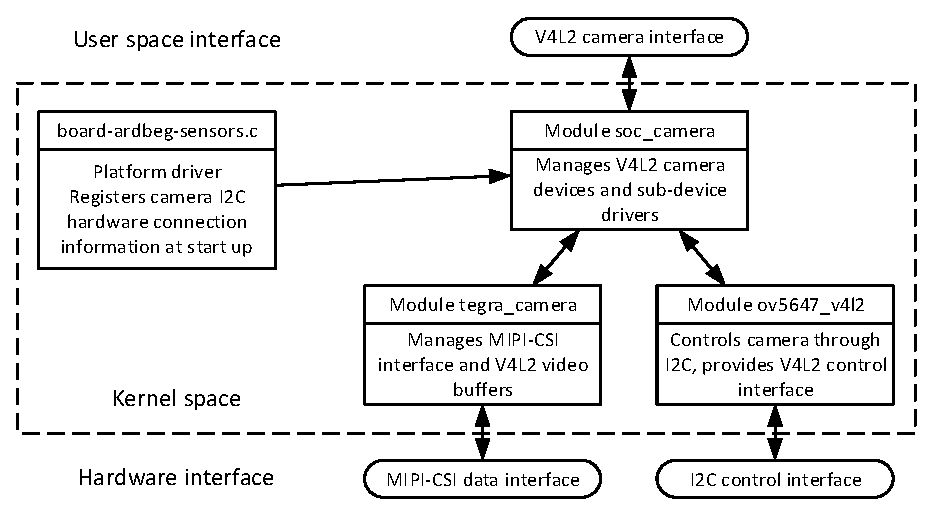
\includegraphics[width=0.7\columnwidth]{drivers}
  \caption{Structure of V4L2 interface drivers on Jetson board.}
  \label{imp:drivers}
\end{figure}

The soc\_camera top module and capture buffer management module are already provided by NVIDIA, therefore only the platform driver and control driver \moda{are} required to be implemented.

For adaptive operation, the driver implemented supports different resolution modes available from the camera and precise frame interval alteration. A special control instruction that can change any of the control registers inside the camera sensor was also developed for debugging and controlling \mdc{purposes}.

\section{Application}

% {\color{red}Application structure, multithreading}
% Bayer pattern handling.
% Multi-threading:
% 	i. Camera thread for camera control, buffer swapping, synchronisation and management etc.
% 	ii. OpenGL preview thread shows the camera output in real time, can be suspended for power saving.
% 	iii. OpenCV worker thread running algorithms.
% 	iv. OpenCV viewing thread.
% 	Display results and handle GUI user input, slow, can be suspended for power saving.

\subsection{Bayer pattern handling}

Initially, for capturing still images and OpenGL video preview, the conversion from Bayer pattern to RGB colour space was implemented. Later in OpenCV processing, it was accomplished through OpenCV's built-in functions directly.

To convert a Bayer pattern image to RGB space, a $3 \times 3$ square of pixels around the target pixel is needed. By averaging surrounding pixels according to \fref{imp:bayer4}, RGB values of each pixel can be approximated.

\begin{figure}[H]
  \centering
  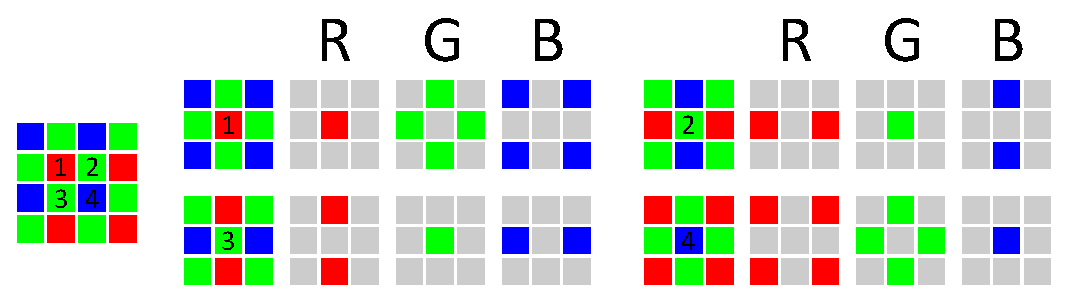
\includegraphics[width=\columnwidth]{bayer4}
  \caption{4 different situations in Bayer pattern to RGB colour space conversion.}
  \label{imp:bayer4}
\end{figure}

\fref{imp:bayer_eg} shows a detailed fraction of a test pattern generated by the camera sensor, and Bayer to RGB colour space conversion result.

\begin{figure}[H]
  \centering
  \subfigure [] {
    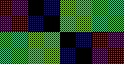
\includegraphics[width=0.4\columnwidth]{bayer_raw}
    \label{imp:bayer_raw}
  }
  \subfigure [] {
    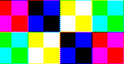
\includegraphics[width=0.4\columnwidth]{bayer_res}
    \label{imp:bayer_res}
  }
  \caption{Test pattern generated by the camera sensor. \subref{imp:bayer_raw} the generated Bayer pattern, \subref{imp:bayer_res} RGB colour space conversion result.}
  \label{imp:bayer_eg}
\end{figure}

% A typical colourful computer image consists of 3 primary colour channels {\color{red}CITE}, which are red, green and blue. However, because of physical and manufacture constrains, most of camera sensors including the camera used in this project have only one intensity sensor per pixel of a specific colour, arranged in a special pattern called Bayer pattern {\color{red}CITE}, therefore image processing algorithm need to be applied to convert or approximate the raw data to produce full colour images. Some of the camera sensors have a built-in image processor that applies the algorithm automatically, but the camera used in this project doesn't have that functionality, therefore the algorithm need to be implemented by the application.

%{\color{red}Some diagrams show how it is done.}

\subsection{Application structure}

An application was developed to receive video stream from \moda{a camera module} or from a testing dataset, then apply OpenCV processing, real-time input and output video preview as well as adaptive camera control. To take the benefits of the heterogeneous architecture more efficiently and overcome issues with buffer updates, the application was implemented using multi-threading approach with inter-thread synchronisation mechanisms.

The main thread in camera mode is responsible for initialisation, camera control, capture buffer synchronisation and management. It allocates several buffers for the camera driver, \mdc{assigns} filled buffers to other processing threads and \mdc{recycles} processed buffers back to camera driver. In dataset mode it reads the sequence of frames, skips frames according to frame rate set by adaptive operation. \modc{The timestamps of video buffers were also recorded, so that exact time between 2 frames can be calculated for adaptive operation.}

After \mdc{obtaining} a frame from video stream, an OpenGL live video preview thread was then used to show the frame to a monitor, independent from the processing algorithm. This thread can be independently stalled so that it would not consume any processing power when analysing performances and power consumptions of algorithms. In camera mode, it will convert the frames received from Bayer pattern format to RGB colour space for rendering onto the screen. This process is done by GPU through OpenGL shaders, therefore is extremely fast, around 200 FPS for $640 \times 480$ resolution if synchronisation with main thread is disabled.

The OpenCV algorithms \mdc{run} on both CPU and GPU, and OpenCV has a \mdc{constraint} that \mdc{is} to view the processed images, the application needs to call a user interface update function that is time consuming but not power intensive, therefore 2 threads \mdc{were} used in a pipeline style in order to speed up the processing. The buffers received from main thread will first go through the processing thread, then pass to the second thread for display on the monitor. The display thread can also be stalled for power saving.

%The OpenCV algorithms runs on both CPU and GPU, therefore to take the full advantages of heterogeneous architecture and run the algorithms as fast as possible, the OpenCV processing runs in a pipelined style through 3 threads. Every buffer received will go through first CPU processing thread, then transferred to GPU processing thread, finally .
%and OpenCV has a constraint that to view the processed image results, the application, so that two OpenCV processing threads was created so that.

Finally, \mdc{there is} an input \mdc{handling} thread for debugging and controlling through command line interface. Most of \mdc{the} time this thread \modc{waits} for user input, therefore won't consume considerable CPU time.

\section{Object detection algorithms}

\subsection{Colour based}

A simple implementation of colour filtering object detection algorithm \cite{MOTBOC.git} was investigated, as shown in \fref{imp:MOTBOC}.

\modc{However, this implementation is very limited. It can only \mdc{detect} objects with single colour, \modc{and it} cannot distinguish the objects from similar background colour. It also relies heavily on manually adjusted colour threshold values for the target model. As a result, this algorithm is very sensitive to the variations of colour from different cameras and environment lighting conditions. Therefore this is not a very adaptable algorithm.} \modc{For example, a} complex environment \modc{that results in} undesired detections \modc{is} shown in \fref{imp:MOTBOC_F}. Background objects that \mdc{have a} similar colour to the desired red objects were detected as foreground red objects\modc{. Some} target objects were not been identified and misclassified because of \mdc{a} slight change in \mdc{the} lighting condition, the objects' colour seen by the camera \mdc{was} no longer inside the colour filters' ranges.

\begin{figure}[H]
  \centering
  \subfigure [] {
    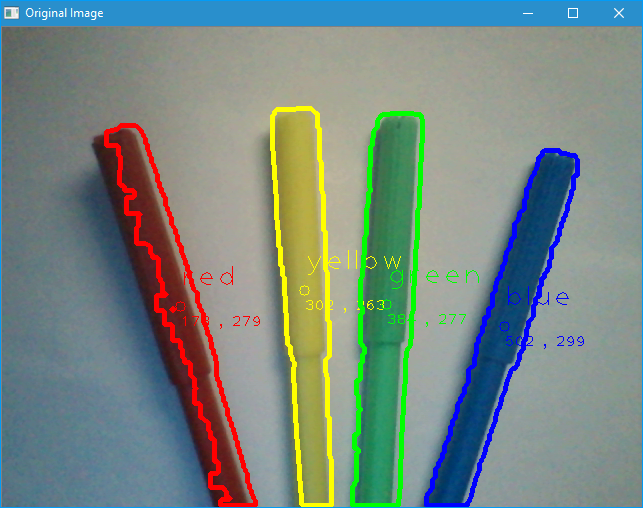
\includegraphics[width=0.4\columnwidth]{MOTBOC_imp}
    \label{imp:MOTBOC_}
  }
  \subfigure [] {
    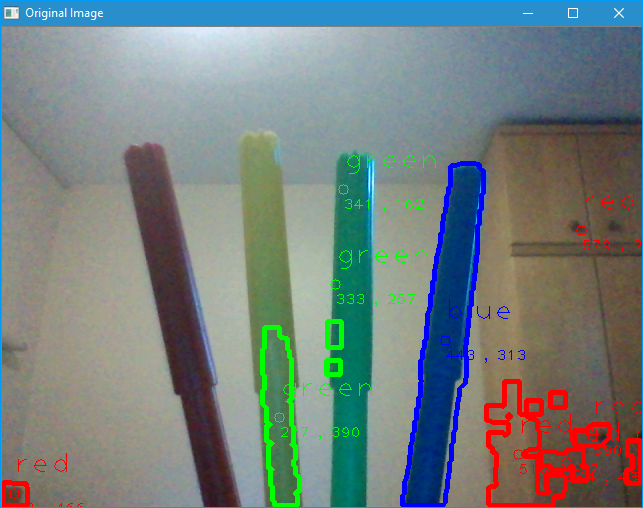
\includegraphics[width=0.4\columnwidth]{MOTBOC_fail}
    \label{imp:MOTBOC_F}
  }
  \caption{Simple multi object tracking based on colour \cite{MOTBOC.git}. \subref{imp:MOTBOC_} ideal situation, \subref{imp:MOTBOC_F} messed up in a complex environment with slightly different lighting condition.}
  \label{imp:MOTBOC}
\end{figure}

\subsection{Circle detection}

OpenCV's implementation of Hough Circle Transform for circle detection was investigated, as shown \mdc{in} \fref{Figure:circles}.

%\fref{Figure:circles} shows the image processed by circle detection, based on OpenCV's implementation of Hough Circle Transform \cite{opencv:hough_circle}.

\begin{figure}[H]
  \centering
  \subfigure [] {
    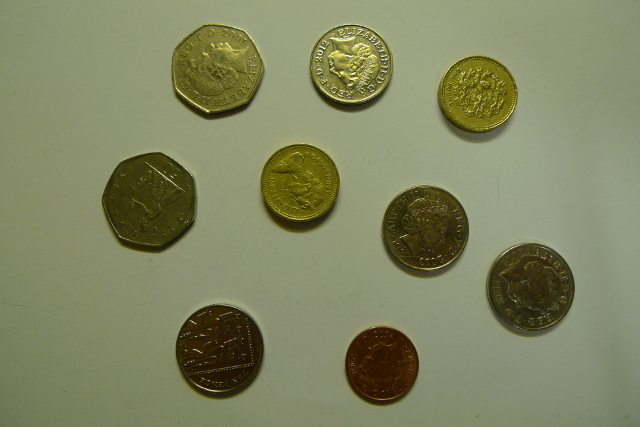
\includegraphics[width=0.45\columnwidth]{simple_original}
    \label{Figure:edges:original}
  }
  \subfigure [] {
    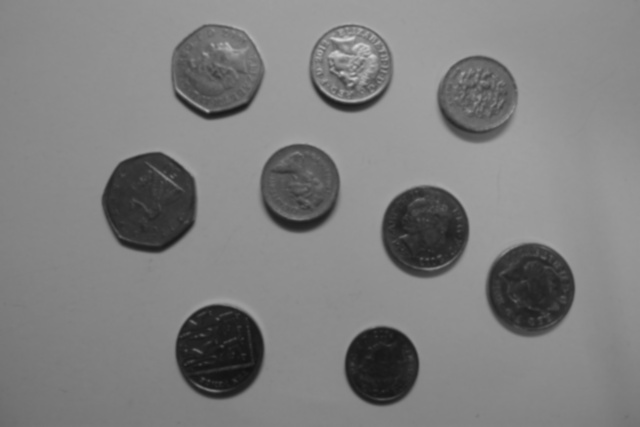
\includegraphics[width=0.45\columnwidth]{simple_blur}
    \label{Figure:edges:blur}
  }
  \subfigure [] {
    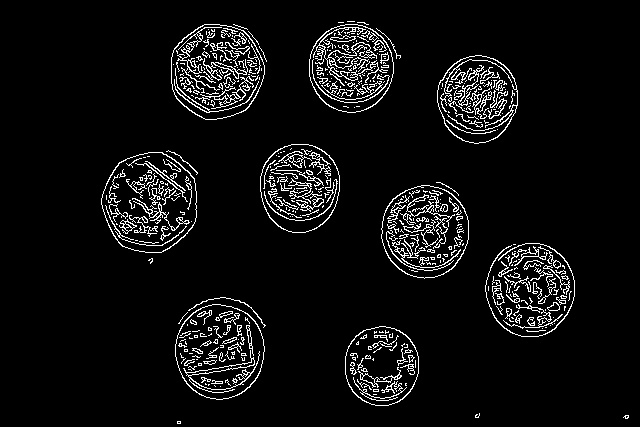
\includegraphics[width=0.45\columnwidth]{simple_edges}
    \label{Figure:edges:edges}
  }
  \subfigure [] {
    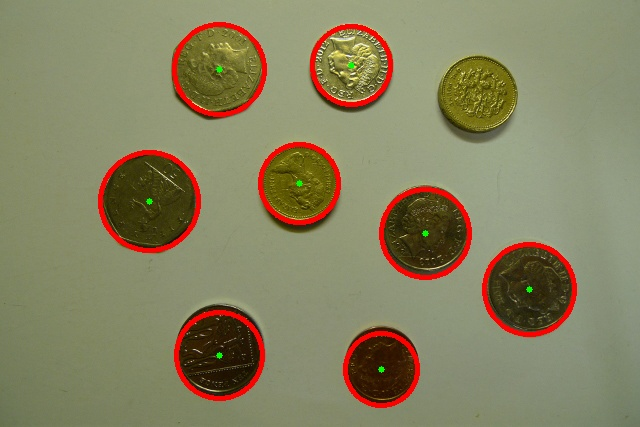
\includegraphics[width=0.45\columnwidth]{simple_circles}
    \label{Figure:edges:circles}
  }
  \caption{Circle detection. \subref{Figure:edges:original} The original image, \subref{Figure:edges:blur} image converted to gray scale and blurred, \subref{Figure:edges:edges} edges extracted, \subref{Figure:edges:circles} circles detected}
  \label{Figure:circles}
\end{figure}

The frame captured from camera (\fref{Figure:edges:original}), was first converted to grey scale then blurred, as shown in \fref{Figure:edges:blur}. Blur or smoothing is necessarily to reduce false object edges that might be detected. Afterwards the object edges in the image \mdc{were} extracted as in \fref{Figure:edges:edges}. Finally \fref{Figure:edges:circles} shows the circles detected by the algorithm.

However, this algorithm is still very limited and inaccurate, as shown \mdc{in} \fref{Figure:circles}, the coin at the top right corner had not been detected, because it appeared to be an ellipse instead of a prefect circle because of \mdc{the} camera perspective. Furthermore, in order to detect multiple geometric shapes, different algorithms would be required for each of the different shapes.

\subsection{Cascade Classifier}

% as shown in \fref{Figure:cc_face}

The OpenCV's cascade classifier implementation \cite{opencv:cc} of face and eye detection \mdc{were} investigated as shown in \fref{Figure:cc_face}.

\begin{figure}[H]
  \centering
  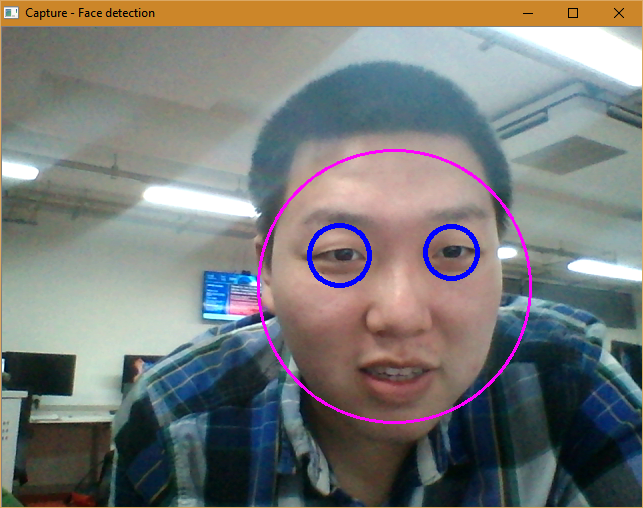
\includegraphics[width=0.6\columnwidth]{cc_imp_face}
  \caption{Face and eye detection cascade classifiers, detected face was circled by pink, whereas detected eyes were circled by blue}
  \label{Figure:cc_face}
\end{figure}

Noticeable frame rate drop \modc{(only about 3 FPS) was} experienced when running the cascade classifier implementation on the testing platform, \mdc{suggesting that} it might not be a suitable algorithm for real-time object tracking application on embedded platforms.

\moda{\subsection{Motion based background subtraction}}

4 out of the 5 best algorithms reviewed by the article \cite{bgs:article} that are available in the BGSLibrary as listed in \tref{Table:bgs} were investigated in this project.

%{\color{red}GPU implementation?}

%\iffalse
\begin{table}[H]
  \centering
  \begin{tabular}{cc}
  \toprule
  \textbf{Method ID} & \textbf{Method name}\\
  \midrule
  MultiLayerBGS & Multi-Layer BGS \\
  MixtureOfGaussianV1BGS & Gaussian Mixture Model \\
  LBAdaptiveSOM & Adaptive SOM \\
  DPWrenGABGS & Gaussian Average \\
  \bottomrule
  \end{tabular}
  \caption{Background substraction algorithms investigated (adapted from \cite{bgslibrary})}
  \label{Table:bgs}
\end{table}
%\fi

%The missing Pixel-Based Adaptive Segmenter (PBAS) algorithm , because the algorithm is based on patented ViBe algorithm, therefore removed from the BGSLibrary to avoid patent issue. However,

The ViBe algorithm from early versions of OpenCV as a non-free add-on module implemented with CUDA runs on GPU, which is also the base of the missing PBAS algotihm, was also investigated.

\fref{Figure:bgs_frame} shows the foreground masks obtained at the same frame index by those 5 algorithms. The dataset used are 2 sample highway surveillance video datasets came with the BGSLibrary \cite{bgslibrary}.

\begin{figure}[htb]
  \centering
  \includegraphics[width=0.3\columnwidth]{bgs_frame/input}
  \includegraphics[width=0.3\columnwidth]{bgs_frame/MultiLayerBGS/mask}
  \includegraphics[width=0.3\columnwidth]{bgs_frame/MixtureOfGaussianV1BGS/mask}
  \includegraphics[width=0.3\columnwidth]{bgs_frame/LBAdaptiveSOM/mask}
  \includegraphics[width=0.3\columnwidth]{bgs_frame/DPWrenGABGS/mask}
  \includegraphics[width=0.3\columnwidth]{bgs_frame/ViBe/mask}


  \includegraphics[width=0.3\columnwidth]{bgs_video/input}
  \includegraphics[width=0.3\columnwidth]{bgs_video/MultiLayerBGS/mask}
  \includegraphics[width=0.3\columnwidth]{bgs_video/MixtureOfGaussianV1BGS/mask}
  \includegraphics[width=0.3\columnwidth]{bgs_video/LBAdaptiveSOM/mask}
  \includegraphics[width=0.3\columnwidth]{bgs_video/DPWrenGABGS/mask}
  \includegraphics[width=0.3\columnwidth]{bgs_video/ViBe/mask}

  \caption{Exemplary frames of results obtained from background subtraction algorithms. Every 2 rows: Input frame, foreground mask obtained by MultiLayerBGS, MixtureOfGaussianV1BGS, LBAdaptiveSOM, DPWrenGABGS and ViBe algorithms.}
  \label{Figure:bgs_frame}
\end{figure}

%{\color{red}Background truth, how to tell best masks?}

The better the \moda{masks match} the moving object, the better the \moda{algorithm} is. It can be seen from \fref{Figure:bgs_frame} that MultiLayerBGS gave \mdc{fewer} holes in the foreground masks, LBAdaptiveSOM had large environment noises, MixtureOfGaussianV1BGS and DPWrenGABGS both produced a large hole in the masks from the second sample dataset. There are some false positions in the foreground mask obtained by ViBe from the first dataset, because the dataset was too short, \moda{so that} the ViBe algorithm \mdc{was} not fully learnt the background model yet. However the masks it computed were still close to the input frame, especially from the second dataset.

\section{Object tracking algorithms}

%Connected component analysis or blob detection (\sref{blob}) and movement tracking (\sref{bg:tracking}) algorithms were not implemented yet.

%A suitable camera module need to be ordered and interfaced afterwards, then implement automatic feedback control of frame rate, cropping and down sampling.

\subsection{Connected component analysis}

Connected component analysis was done as shown \mdc{in} \fref{imp:cca}. The baseline highway sample dataset from CDNET \cite{goyette2012changedetection} was used, it has 1700 frames, 30 frames per second and the resolution is $320 \times 240$. The ViBe background subtraction algorithm was used to extract foreground masks as shown \mdc{in} \fref{imp:cca:mask}, for connected component analysis algorithm to evaluate. OpenCV's find contours \modc{function was} used to extract the blobs. However, in order for it to work properly, the masks need to be cleaned up first. This was done by applying a find contours function first, filtering out small contours that are mostly likely noises, then redraw the contours. That may still \mdc{leave} unclosed holes, therefore a Morphology transformation \cite{serra1982image} was applied afterwards to close those holes. \fref{imp:cca:mask2} shows the mask been cleaned up. Finally, apply the find contours function to the enhanced foreground mask, results in numbers of contours, outlined on the input frame shown \mdc{in} \fref{imp:cca:drawing}.

\begin{figure}[htb]
  \centering
  \subfigure [] {
    \includegraphics[width=0.4\columnwidth]{contours/input}
    \label{imp:cca:input}
  }
  \subfigure [] {
    \includegraphics[width=0.4\columnwidth]{contours/mask}
    \label{imp:cca:mask}
  }
  \subfigure [] {
    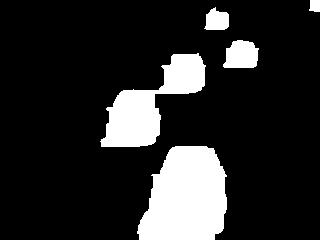
\includegraphics[width=0.4\columnwidth]{contours/img_mask}
    \label{imp:cca:mask2}
  }
  \subfigure [] {
    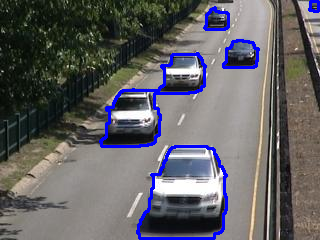
\includegraphics[width=0.4\columnwidth]{contours/drawing}
    \label{imp:cca:drawing}
  }
  \caption{Contours extracted from foreground masks. \subref{imp:cca:input} input frame, \subref{imp:cca:mask} foreground mask extracted by ViBe, \subref{imp:cca:mask2} enhanced foreground mask, \subref{imp:cca:drawing} contours (blobs) extracted}
  \label{imp:cca}
\end{figure}

%\subsection{Continuously Adaptive Meanshift}

\subsection{Optical flow}

\fref{imp:of} shows exemplary sparse set optical flow tracking result between 2 frames. The frames were taken from the baseline highway dataset from CDNET \cite{goyette2012changedetection}, but are 8 frames apart, in order to investigate how well the optical flow algorithm works when \modc{objects travel} too fast, \modc{move} a long distance between adjacent frames.

\begin{figure}[htb]
  \centering
  \subfigure [] {
    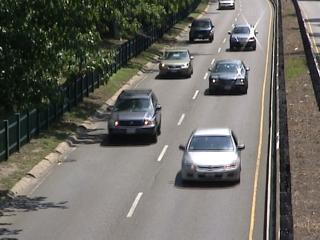
\includegraphics[width=0.3\columnwidth]{optical/between/prev}
    \label{imp:of:prev}
  }
  \iffalse
  \subfigure [] {
    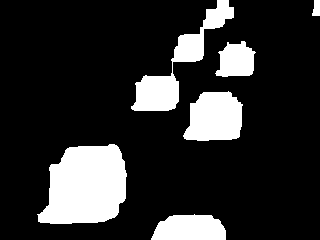
\includegraphics[width=0.3\columnwidth]{optical/between/prev_mask2}
    \label{imp:of:prev_mask}
  }
  \fi
  \subfigure [] {
    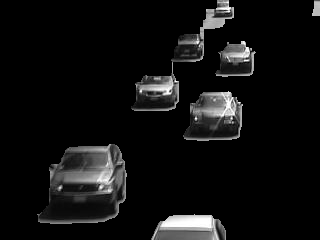
\includegraphics[width=0.3\columnwidth]{optical/between/prev_input_of}
    \label{imp:of:prev_input_of}
  }
  \subfigure [] {
    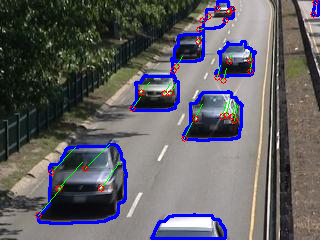
\includegraphics[width=0.3\columnwidth]{optical/between/prev_drawing}
    \label{imp:of:prev_drawing}
  }
  \subfigure [] {
    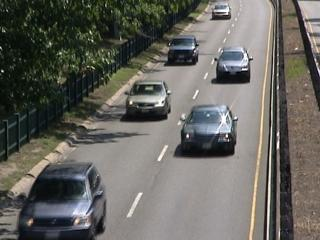
\includegraphics[width=0.3\columnwidth]{optical/between/next}
    \label{imp:of:next}
  }
  \subfigure [] {
    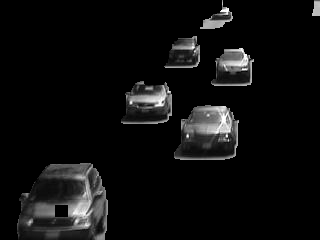
\includegraphics[width=0.3\columnwidth]{optical/between/next_input_of}
    \label{imp:of:next_input_of}
  }
  \subfigure [] {
    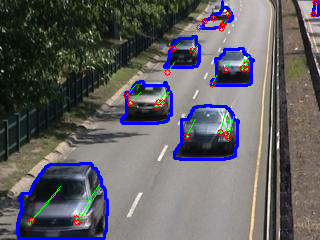
\includegraphics[width=0.3\columnwidth]{optical/between/next_drawing}
    \label{imp:of:next_drawing}
  }
  \caption{Sparse set optical flow tracking between 2 frames. \subref{imp:of:prev} previous frame, \subref{imp:of:prev_input_of} masked previous frame, \subref{imp:of:prev_drawing} optical tracking result at the previous frame, \subref{imp:of:next} next frame, \subref{imp:of:next_input_of} masked next frame, \subref{imp:of:next_drawing} optical flow tracking result at the next frame. {\color{red}Red circles}: Destinations of feature points generated from previous frame; {\color{dkgreen}Green lines}: Movements of the feature points; {\color{blue}Blue \modc{outlines}}: Object blobs extracted from foreground mask.}
  \label{imp:of}
\end{figure}

The feature points were taken from corner points along the edges of contours extracted by background subtraction algorithm. The input frames were also masked by the foreground masks as shown \mdc{in} \fref{imp:of:prev_input_of} and \fref{imp:of:next_input_of} to reduce possible distractions to the algorithm.

However, sometimes the optical flow algorithm may \mdc{give} incorrect tracking results, for example the 2 frames shown in \fref{imp:of:error}. To filtering out those occasions, it is necessary to estimate the maximum possible velocity of objects moving in the scene.

\begin{figure}[htb]
  \centering
  \subfigure [] {
    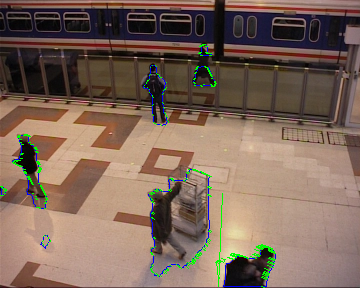
\includegraphics[width=0.45\columnwidth]{optical/error/000170_drawing}
    \label{imp:of:error:1}
  }
  \subfigure [] {
    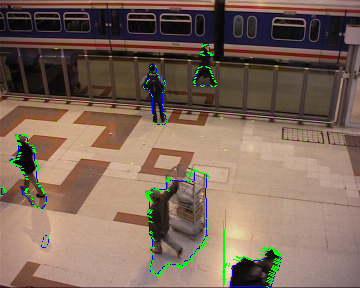
\includegraphics[width=0.45\columnwidth]{optical/error/000171_drawing}
    \label{imp:of:error:2}
  }
  \caption{Situation when optical flow gives unrealistic results for 2 frames from CDNET baseline PETS2006 dataset. {\color{dkgreen}Green lines}: Movements of the feature points; {\color{blue}Blue \modc{outlines}}: Object blobs extracted from foreground mask.}
  \label{imp:of:error}
\end{figure}

By relating the destination of movements of feature points from blobs in previous frame to blobs detected in the next frame, the blobs can be tracked between frames. However this is not required for \modb{obtaining} the \modb{highest} speed of \modb{objects moving between frames, which is the input the adaptive operation depends on. Implementing} this would \modb{also} require lots of efforts for statistic computation to filtering out incorrect tracking results, point in polygon testing \modb{algorithm} and blob management, therefore was considered as further work.

\section{\modc{Adaptive \modb{energy} saving operation}}

Adaptive energy saving operation was done by varying input video stream frame rate based on object tracking results, a feedback loop as previous illustrated in the system block diagram (\fref{block}).

\subsection{Parameter metrics}
\label{imp:ada:metric}

\mdd{A few parameter metrics are required for an \modd{optimal} performance in a particular scenario. They are} listed in \tref{imp:ada:par}.

\begin{table}[H]
  \centering
  \begin{tabular}{cc}
  \toprule
  \textbf{Parameter metric} \\
  \midrule
  Maximum possible object moving speed. \\
  Typical object sizes. \\
  Typical distances between objects. \\
  Active area masks. \\
  Minimum acceptable frame rate. \\
  Maximum possible frame rate. \\
  \bottomrule
  \end{tabular}
  \caption{Parameter metrics required for adaptive energy saving operation}
  \label{imp:ada:par}
\end{table}

The basic one is the maximum possible moving speed of any objects and parts of objects in the scenario. It is used to determine all other parameters.

Typical object sizes, distances between objects and active area masks are used to optimise foreground mask filtering, so that noises and movements caused by other unrelated objects can be filtered out as much as possible. They are irrelevant to the optical flow tracking algorithm, because the algorithm is tracking feature points around blobs \mdd{rather than} shapes of blobs.

The minimum frame rate is determined by \eref{f_min}, so that movement of any object will not overtake the tracking window, therefore most likely keep \mdd{being} tracked. It is also limited by minimum response rate required in an application.

\begin{equation}
	f_{min} = \frac{\text{Maximum object speed}}{\text{Optical flow optimum tracking length}}
	\label{f_min}
\end{equation}

The maximum frame rate is only limited by algorithm computation speed and hardware limitations.

\subsection{Frame rate adaptation}

Having calculated the maximum movement distance of feature points between adjacent frames, the frame rate is then calculated \mdd{by} \eref{f_rate}. The frame interval will then be adjusted according to this by the main thread.

\begin{equation}
	f = \frac{\text{Maximum movement distance}}{\text{Optical flow optimum tracking length} \times \text{Time between frames}}
	\label{f_rate}
\end{equation}

%{\color{red}Implementation? BOOM}

\fref{imp:ada:ex} shows a sequence of frames evaluated from the CDNET baseline highway dataset. The frame indices are not continuous due to the adaptive operation applied. It can be seen from the sequence of frames that the change of frame rate (\fref{imp:ada:ex:part}) is clearly related to the speeds of objects. \modd{The maxima of object travelling distances indicated by the green lines are almost the same.}

\begin{figure*}[htb]
  \centering
  \subfigure[Frame 1602]{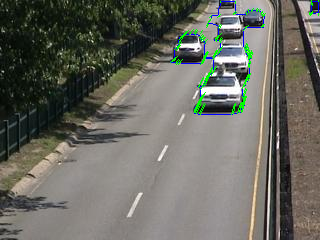
\includegraphics[width=0.23\columnwidth]{adaptive/example/001602_drawing}}
  \subfigure[Frame 1608]{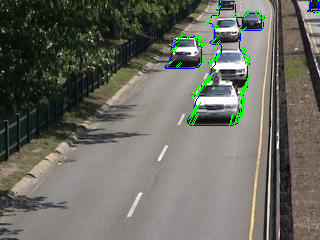
\includegraphics[width=0.23\columnwidth]{adaptive/example/001608_drawing}}
  \subfigure[Frame 1614]{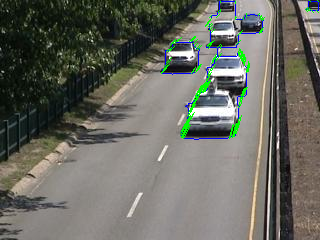
\includegraphics[width=0.23\columnwidth]{adaptive/example/001614_drawing}}
  \subfigure[Frame 1620]{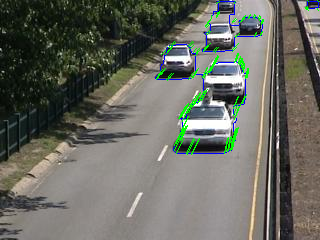
\includegraphics[width=0.23\columnwidth]{adaptive/example/001620_drawing}}
  \subfigure[Frame 1626]{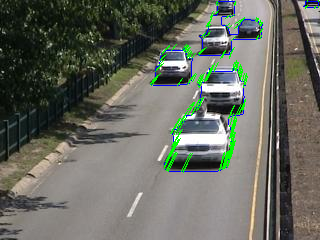
\includegraphics[width=0.23\columnwidth]{adaptive/example/001626_drawing}}
  \subfigure[Frame 1632]{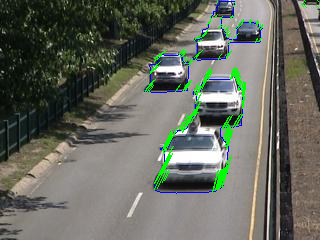
\includegraphics[width=0.23\columnwidth]{adaptive/example/001632_drawing}}
  \subfigure[Frame 1638]{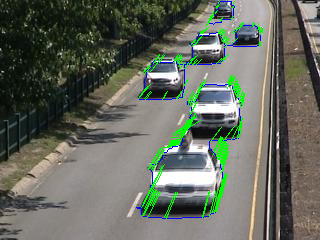
\includegraphics[width=0.23\columnwidth]{adaptive/example/001638_drawing}}
  \subfigure[Frame 1644]{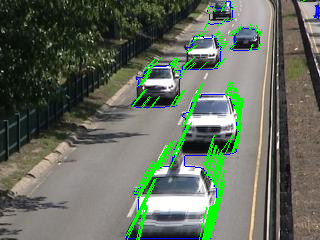
\includegraphics[width=0.23\columnwidth]{adaptive/example/001644_drawing}}
  \subfigure[Frame 1648]{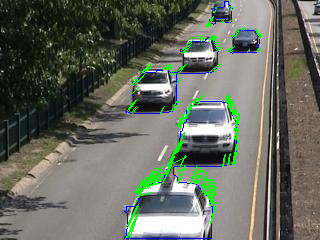
\includegraphics[width=0.23\columnwidth]{adaptive/example/001648_drawing}}
  \subfigure[Frame 1651]{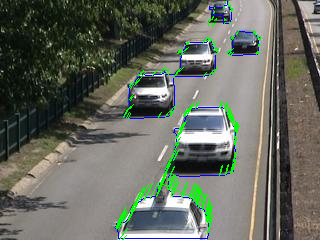
\includegraphics[width=0.23\columnwidth]{adaptive/example/001651_drawing}}
  \subfigure[Frame 1654]{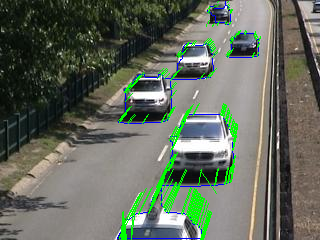
\includegraphics[width=0.23\columnwidth]{adaptive/example/001654_drawing}}
  \subfigure[Frame 1656]{\includegraphics[width=0.23\columnwidth]{adaptive/example/001656_drawing}}
  \subfigure[Changes of frame rate through the sequence shown above]{
    \includegraphics[width=0.7\columnwidth]{adaptive/example/fps_part}
    \label{imp:ada:ex:part}
  }
  \subfigure[Changes of frame rate through the entire dataset]{
    \includegraphics[width=\columnwidth]{adaptive/example/fps_all}
    \label{imp:ada:ex:all}
  }
  \caption{Frames evaluated from the highway dataset after applied adaptive operation.}
  \label{imp:ada:ex}
\end{figure*}

%\todo{Update the frames}

The changes of frame rate through the entire dataset are shown in \fref{imp:ada:ex:all}. Most of the time frame rate is below 10 FPS, \mdd{resulting} in only 274 out of 1700 frames in the dataset \mdd{being} evaluated\mdd{. This} saves a lot of computation.

%\section{Video stream dataset}
